\documentclass{article}
\usepackage{tikz,pgfplots}
\begin{document}
\vspace{1cm}
\section{Plot the true stress-strain curve}
\vspace{1cm}
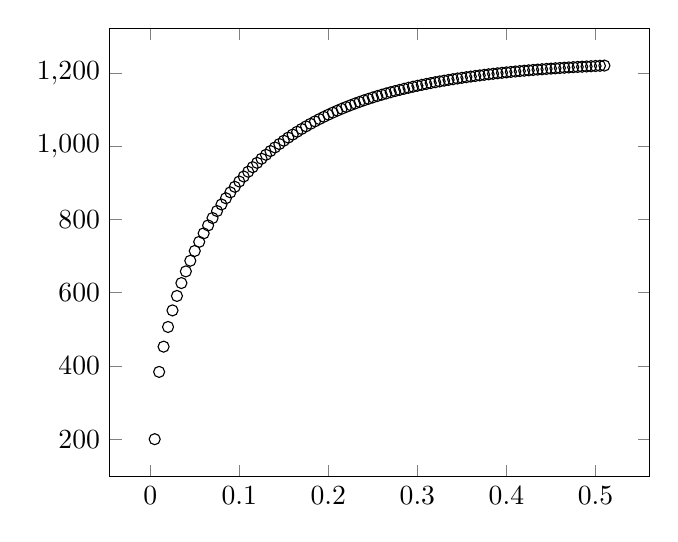
\begin{tikzpicture}
\begin{axis}[%
scatter/classes={%
    a={mark=o,draw=black}}]
\addplot[scatter,only marks,%
    scatter src=explicit symbolic]%
table[meta=label] {
x y label
0.005 200 a
0.01 383.651 a
0.015 452.539 a
0.02 506.295 a
0.025 551.502 a
0.03 590.942 a
0.035 626.109 a
0.04 657.925 a
0.045 687.009 a
0.05 713.8 a
0.055 738.627 a
0.06 761.745 a
0.065 783.354 a
0.07 803.617 a
0.075 822.671 a
0.08 840.629 a
0.085 857.587 a
0.09 873.629 a
0.095 888.828 a
0.1 903.247 a
0.105 916.942 a
0.11 929.965 a
0.115 942.359 a
0.12 954.166 a
0.125 965.423 a
0.13 976.161 a
0.135 986.413 a
0.14 996.206 a
0.145 1005.57 a
0.15 1014.52 a
0.155 1023.08 a
0.16 1031.27 a
0.165 1039.12 a
0.17 1046.64 a
0.175 1053.84 a
0.18 1060.74 a
0.185 1067.36 a
0.19 1073.71 a
0.195 1079.8 a
0.2 1085.65 a
0.205 1091.26 a
0.21 1096.64 a
0.215 1101.82 a
0.22 1106.78 a
0.225 1111.55 a
0.23 1116.14 a
0.235 1120.54 a
0.24 1124.78 a
0.245 1128.85 a
0.25 1132.76 a
0.255 1136.52 a
0.26 1140.14 a
0.265 1143.62 a
0.27 1146.97 a
0.275 1150.19 a
0.28 1153.28 a
0.285 1156.26 a
0.29 1159.13 a
0.295 1161.89 a
0.3 1164.55 a
0.305 1167.1 a
0.31 1169.57 a
0.315 1171.93 a
0.32 1174.22 a
0.325 1176.41 a
0.33 1178.53 a
0.335 1180.56 a
0.34 1182.52 a
0.345 1184.41 a
0.35 1186.23 a
0.355 1187.98 a
0.36 1189.67 a
0.365 1191.3 a
0.37 1192.86 a
0.375 1194.37 a
0.38 1195.82 a
0.385 1197.22 a
0.39 1198.57 a
0.395 1199.87 a
0.4 1201.12 a
0.405 1202.33 a
0.41 1203.49 a
0.415 1204.61 a
0.42 1205.69 a
0.425 1206.73 a
0.43 1207.74 a
0.435 1208.7 a
0.44 1209.63 a
0.445 1210.53 a
0.45 1211.4 a
0.455 1212.23 a
0.46 1213.03 a
0.465 1213.81 a
0.47 1214.55 a
0.475 1215.27 a
0.48 1215.97 a
0.485 1216.64 a
0.49 1217.28 a
0.495 1217.9 a
0.5 1218.5 a
0.505 1219.08 a
0.51 1219.64 a
};
\end{axis}
\end{tikzpicture} \par 
(Mecking-Kocks Model with Glide only, D=1e-06m $\rho$=1e+13)
\end{document}
